\documentclass[11pt, a4paper]{report}
%\documentclass[11pt,a4paper,oneside]{report}

%Packages
\usepackage[hungarian]{babel}
\usepackage[utf8]{inputenc}
\usepackage{graphicx}
%
\usepackage{hyperref}
\usepackage{wrapfig}
\usepackage{subfigure }
\usepackage[margin=80pt]{geometry}
\usepackage{geometry}
\usepackage{amsmath}
\usepackage{tabularx}
\usepackage{tabulary}
%\usepackage{url}
\usepackage{multicol}
\usepackage{multirow}
\usepackage{setspace}
\usepackage[table,xcdraw]{xcolor}
%\usepackage[acronym]{glossaries}
\usepackage{longtable}
\usepackage{titlesec}



\usepackage[procnames]{listings}
\usepackage{color}


\definecolor{keywords}{RGB}{255,0,90}
\definecolor{green}{RGB}{0,0,113}
\definecolor{red}{RGB}{160,0,0}
\definecolor{comments}{RGB}{0,150,0}
 
\lstset{language=Python, 
        basicstyle=\ttfamily\small, 
        keywordstyle=\color{keywords},
        commentstyle=\color{comments},
        stringstyle=\color{red},
        showstringspaces=false,
        identifierstyle=\color{green},
        procnamekeys={def,class}}

\pagestyle{plain}
\setlength{\parindent}{12pt} % magyar nyelvû dokumentumokban jellemzõ
\setlength{\parskip}{0pt}    % magyar nyelvû dokumentumokban jellemzõ
\frenchspacing
\setlength{\columnsep}{1cm}
\linespread{1.5}

\includeonly{
	cimlap,
	eloszo,
	fejezet1,
	zaras,
	fuggelek,
}
%%%%%%%%%%%%%%%%%%%%%%%%%%%%%%%%%%%%%%%%%


\begin{document}

%--------------------------------------------------------------------------------------
%	The title page
%--------------------------------------------------------------------------------------
\begin{titlepage}
\begin{center}

\includegraphics[width=60mm,keepaspectratio]{figures/BMElogo.png}\\
\vspace{0.3cm}
\textbf{Budapesti Műszaki és Gazdaságtudományi Egyetem}\\
\textmd{Villamosmérnöki és Informatikai Kar}\\
\textmd{Távközlési és Médiainformatikai Tanszék}\\[2.5cm]

\vspace{0.5cm}
\textsc{\LARGE Diplomaterv 1}\\[0.1cm]
\textsc{2015/16. tanév, 2. félév}\\[1.5cm]
\vspace{0.4cm}
{\huge \bfseries Automatizált internetes mérések}\\[5cm]

\begin{tabular}{cc}
 \makebox[7cm]{\emph{Készítette}} & \makebox[7cm]{\emph{Konzulens}} \\
 \makebox[7cm]{Horváth Rudolf} & \makebox[7cm]{Dr Heszberger Zalán}
\\
 \makebox[7cm]{rudolf.official@gmail.com} & \makebox[7cm]{heszberger@tmit.bme.hu}
 \\
 \makebox[7cm]{TS48JK} & \makebox[7cm]{}
\end{tabular}

\vfill
{\large \today}
\end{center}
\end{titlepage}




\chapter*{Kivonat}\addcontentsline{toc}{chapter}{Kivonat}
%1 oldalas összefoglalása a munkának \textbf{Magyarul}.

Az internet olyan kulcsfontosságú infrastruktúra napjainkban, amelynek fontos ismerni az állapotát és viselkedését. Ezen Diplomamunka az internetes útvonalak vizsgálatával foglalkozik.
Egy automatizált Internetes mérési rendszer készült ennek érdekében, amely a PlanetLab szervezet gépeit felhasználva méréseket végez és monitorozza az internet általuk látható részeit. A mérési rendszer több mérési funkcióval rendelkezik. A begyűjtött adatok több feldolgozási folyamaton mennek keresztül, melyek egyik kimenete például útvonal változásokat elemez. A megbízható adatszolgáltatás érdekében a mérési rendszer folyamatos és hibatűrő működésre lett tervezve, felügyeleti funkciókkal kiegészítve. A felhasznált technológiák és az elkészült szoftverkomponensek nyílt forráskódú licensszel rendelkeznek, így mások is használhatják azokat, illetve bővíthetik saját fejlesztéseikkel.
A begyűjtött adatok előzetes elemzése bemutatta, hogy a mérési rendszer valóban képes megfigyeléseket tenni az Internetes útvonalakra vonatkozóan. A publikált eredmények és eszközök értéket jelenthetnek minden internetes méréssel foglalkozó csoportnak.

\chapter*{Abstract}\addcontentsline{toc}{chapter}{Abstract}

Today, the Internet is a key infrastructure, it is important to know the behavior and current conditions of it. This Thesis deals with Internet route measurements, which helps to better understand, and tries to answer these question.
For this purpose, an automated measurement system was developed, which carries out internet measurements with the help of the PlanetLab network. The system is monitoring the parts of the internet seen by the nodes of the network. The collected measurements are stored and processed by multiple pipelines for different purposes, like route evolution observation. To provide a reliable data feed, the measurement system was designed for continuous and fault tolerant operation, extended with operational supervision functions. The used and developed technologies are accessible under Open-source licenses. Anybody has access to them and can further develop new components to it.
The collected data and its preliminary analysis demonstrated, that the measurement system can provide insights into the behavior of Internet routes. The publicized results and tools can have a real value for groups interested in internet measurements.


%Régi:
%Az internet olyan kulcsfontosságú infrastruktúra napjainkban, amelynek fontos ismerni az állapotát és viselkedését. Ezen Diplomamunka az internetes útvonalak vizsgálatával foglalkozik. Egy automatizált Internetes mérési rendszer készült ennek érdekében, amely a PlanetLab szervezet gépeit felhasználva méréseket végez és monitorozza az internet általuk látható részeit. A mérési rendszer több mérési funkcióval rendelkezik, a begyűjtött adatok több feldolgozási folyamaton mennek keresztül a jobb információprezentálás érdekében. Mindezeken felül a mérési rendszer folyamatos, megbízható és hibatűrő működésre lett tervezve.


%\chapter*{Abstract}\addcontentsline{toc}{chapter}{Abstract}
%1 oldalas összefoglalása a munkának \textbf{Angolul}.

%\chapter*{Bevezető}\addcontentsline{toc}{chapter}{Bevezető}
%A kivonatnál bővebb leírás miről szól a dolgozat.




%Önlab2 előszava:
%Az internet olyan kulcsfontosságú infrastruktúra napjainkban, amelynek fontos ismerni az állapotát és viselkedését. Önálló laboratóriumi feladatom során az internetes útvonalak automatizált mérésével és értelmezésével foglalkoztam. Az általam készített és továbbfejlesztett mérőrendszer a PlanetLab szervezet gépeit felhasználva méréseket végez és monitorozza az internet általuk látható részeit. Munkám során több új mérési funkciót fejlesztettem, valamint az új mérési forgatókönyvek implementálását egyszerűvé és kényelmessé tettem, a folyamatosan gyűlő adatokat könnyen feldolgozható formába alakítottam. Mindezeken felül fontos szempont volt a folyamatos, megbízható és hibatűrő működés, valamint a mérések felügyelete.



%%%%%%%%%%%%%%%%%%%%%%%%%%%%%%%%%%%%%%%%%%%%%%%%%%%%%%
%Elvégzett munka tartalma:

%Migráltam az adatmentés és adatkezelést MySQL-ről MongoDB-re, mert jobbnak tűnt, hogy nem merevek az adatstruktúrák és megférnek egymás mellett a régebbi formátumú adatok és a kísérleti, friss adatok is.
%A folyamatos futtatás érdekében a RedHat Openshift felhős platformjára telepítettem az egész mérést, így ott folyamatosan elindul, fut, ment egyből adatbázisba. Valamint egy honlapon mutat pár visszajelzést, hogyan áll: http://python-limiere.rhcloud.com/
%Több hibát javítottam, amiknek hála szinte bármilyen (akár új, váratlan) hiba előfordulásakor folytatják a mérést. Alapvetően függetlenítettem az egyes folyamatokat, amik felügyelni tudják a másikat és szükség esetén leállítják, újraindítják azokat.
%A hibák és a futások felügyeletéhez szinte mindenhol bevezettem a logolást, így végigkövethető hol milyen hiba miatt nem volt sikeres a mérés.
%Eddig csak traceroute mérés volt, de ezt kiegészítettem az iperf méréssel.
%Ennek nyomán pedig egy viszonylag szép általánosan bevethető eljárást készítettem, ahol különböző parancsok időzített, egymáshoz illesztett indítását lehet levezetni. Például ugye a párhuzamos méréshez kellett ez.
%Végül ugye elkészítettem az éllistából álló adatbázist amiben minden elérhető adat rendelkezésre áll (időpont, két ip cím, késleltetés, jitter ...)


%%%%%%%%%%%%%%%%%%%%%%%%%%%%%%%%%%%%%%%%%%%%%%%%%%%%%%
%Önlab2 eredeti kiírás:
%A labortéma a Forgalmi mérések az Interneten c. önálló labor kiírás testvértémája, és első sorban a mért adatok elemzését célozza: A laborfeladat célja méréseket végezni a nagy Interneten. A feladathoz az elmúl félévben korábbi önálló labormunka keretében készültek rövidebb python alapú szkriptek melyek az Interneten elérhető számos gép közötti forgalmat ill. annak viselkedését (pl. útvonalválasztási jellemzőit) mérik. Feladat lehet ezen mérések kivitelezése esetleg ha szükséges a scriptek továbbfejelsztése. A méréseket szeretnénk kielemezni, és következtetéseket levonni belőle a nagy Internet kinézetére és viselkedésére vonatkozólag.

%%%%%%%%%%%%%%%%%%%%%%%%%%%%%%%%%%%%%%%%%%%%%%%%%%%%%%
%Önlab1 előszava:
%Az internet fejlődése napjainkban nehezen követhető, hiába az alapjait alkotó protokollok alapos ismerete. A megvalósított hálózatok üzleti, jogi vagy természetes eredetű okok miatt sokszor eltérnek az eredetileg elképzelttől.
%Ezért az internet továbbfejlesztésének/újratervezésének egyik fontos feltétele a valóságos hálózatok ismerete. 
%
%Önálló laboratóriumi munkám során, hogy tapasztalatokat gyűjtsek az internet felépítéséről és a vizsgálatához szükséges technológiákról, méréseket végeztem a PlanetLab szervezet által elérhető számítógépek segítségével. A mérések célja az internet csomópontjai között lévő útvonalak és ezen útvonalak által létrehozott gráf feltérképezése és vizsgálata volt.


%------------------------------------------
%----------  Feladat kiírás  --------------
%\vspace{1.4cm}

%\noindent
%\textsc{\Huge \textbf{Feladat}}

%\bigskip
%%\indent

%%Önlab1 Feladat leírása
%A félév során a hallgató feladata a korábbi önálló laboratóriumi munkájának folytatása. A PlanetLab teszthálózat gépeinek segítségével végez internetes méréseket és tovább fejleszti azokat. A mérési eredményeket szűri és könnyen feldolgozható formában tárolja. Végül elemzéseket végez rajtuk.

%%%%%%%%%%%%%%%%%%%%%%%%%%%%%%%%%%%%%%%%%%%%%%%%%%%%%%
%Önlab1 Feladat leíása:
%A félév során a hallgató feladata az internet valóságos működésének és felépítésének vizsgálata. A témához tartozó irodalmakat tanulmányozza, majd a PlanetLab teszthálózaton automatizált méréseket folytat. Az így kapott mérési eredményeket feldolgozza és elemzi.




%%%%%%%%%%%%%%%%%%%%%%%%%%%%%%%%%%%%%%%%%%%%%%%%%%%%%%
%Önlab2 félév eleji feladat leírása:
%Féléves feladat:
%Internetes mérések tervezése, kivitelezése és elemzése,
%amely az internet felépítését elemzi
%és megvizsgálja az mptcp protokoll lehetséges előnyeit.
%
%A munka ütemezése:
%
%Előkészületek:
%4-5. hét  A kivitelezendő mérések kidolgozása. Teszt mérések végzése.
%
%Mérnöki munkavégzés:
%6-7. hét  Folyamatos mérések végzése és azok felügyelete.
%
%8-12.hét  A mérési eredmények aggregálása, feldolgozása és vizsgálata
%
%Dokumentálás:
%13.  hét  Felkészülés a szóbeli és írásbeli beszámolóra.




%%%%%%%%%%%%%%%%%%%%%%%%%%%%%%%%%%%%%%%%%%%%%%%%%%%%%
%Önlab1 eredeti kiírás:
%Az internet gyerekbetegségeinek tüneti kezelése mind komolyabb feladatot ró a szakemberekre. Egyre többen látják a megoldást az internet alapoktól való újragondolásában. Az általunk vizsgált kérdések érintik többek között a címzést, címkiosztást, útvonalválasztást, topológiát valamint az internet erősen elosztott és dinamikus jellegéből adodó nehézségeket. A laborfeladat célja megismerni az internet újragondolásának lehetséges új irányvonalait, ismertebb kezdeményezéseit. A félév második felében lehetőség nyílna alternatív hálózati technológiák elméleti és szimulációs és teszthálózati vizsgálatára ill. prototípus építésére.



\tableofcontents

\chapter{Fejezet}


Lényegi tartalom (25-30 oldal):
Mérési elrendezés (5 oldal): traceroute, iperf, mérési forgatókönyvek, PlanetLab
Fejlesztési megfontolások (8-10 oldal): python, mongodb, logolás, email küldés, weboldal, hibák függetlenítése, megbízhatóságnövelő megfontolások
Mérési eredmények (7-10 oldal): kinyert mérések tartalma(delay, jitter, link, AS info, Geolocation), mérések mennyisége, mérések minősége
Adattisztítás, feldolgozás (5 oldal): Hibák kiszűrése, gráf reprezentálás, statisztikák



\section{Szekció}


%%%%%%%%%%%%%%%%%%%%%%%%%%%%%%%%%%%%%%%%%%%%%%%%%
% Címszavakban a tartalom:
%
% 

\chapter{Összefoglalás}
1-2 oldal
%Dolgozatom zárásaként összegyűjtöm az elvégzett munkák eredményeit, a főbb szerzett tapasztalatokat, valamint kitekintést nyújtok az elért eredmények felhasználására és a további kutatási lehetőségekre.

\section{Elért eredmények}

%A féléves munkám során továbbfejlesztettem a már meglévő mérési rendszert, amely a PlanetLab hálózatán elérhető gépeken végez internetes méréseket. A mérési folyamat megbízhatóságát nagyban növeltem és az eredmények feldolgozásában is nagy előrehaladást értem el. Az általam fejlesztett rendszerhez könnyen hozzáadható újabb, akár komplexebb mérés. A mérési folyamat teljesen monitorozható az általa szolgáltatott webes honlap segítségével és a lehetséges hibák könnyen kideríthetővé váltak. A kapott mérési eredmények pedig még kezdetlegesen, de megtekinthetőek szintén a webes interfészen.


%--------------------
%A féléves munkám során elmélyítettem az internet felépítéséről és működéséről való ismereteimet, gyakorlatot szereztem a PlanetLab teszthálózat ezres nagyságrendű számítógépeinek elérésében, amelyeken automatizált méréseket végeztem. Tapasztalatokat szereztem nagyobb adatbázisok menedzselésében, valamint a nagy gráfok kezelésébe és ábrázolásába is betekintést nyertem.
%
%Munkám gyümölcseként létrehoztam egy folyamatosan bővülő adatbázist az internetes útvonalakról, amelynek vizsgálatát a félév során csak megkezdeni tudtam.


\section{Továbbhaladási lehetőségek}
%A mérést végző rendszeren már nem szükségesek komoly fejlesztések. A mérési eredményeket feldolgozó eljárásokat fontos a jövőben továbbfejleszteni, valamint a webes interfész felhasználóbaráttá tétele. Az eddig elért munkát Diplomatervként tervezem folytatni, de mint Haja Dávid szakdolgozata is bizonyítja más projektmunkák is könnyen be tudnak csatlakozni a fejlesztésekbe. A bekapcsolódási lehetőségeket konzulensemmel igyekszünk újabb témakiírásokkal támogatni.

%--------------------
%A féléves munka folytatásaként fontosnak tartanám az eddig felhalmozott adatok jobb feldolgozását, és a gráf reprezentációk fejlesztését. Ezeken felül a mérés kibővítésére tennék javaslatokat, mint a mérési időpontok pontosítása (jelenleg a napon belüli bontás nem megfelelő), több cél IP cím hozzáadása, valamint az útvonal szimmetriájának vizsgálata érdekében az útvonalak két oldalról történő mérése.

%%%%%%%%%%%%%%%%%%%%%%%%%%%%%%%%%%%%%%%%%%%%%%%%%
%Önlab1 megjegyzések
%Az eddigi mérési eredményeket úgy gondolom több módon is fel lehetne dolgozni. Egyik magától értetődő cél lehetne az útvonalak késleltetésének, fontosságának (a csomópontok közötti legrövidebb útvonalakban hányszor fordul elő) reprezentálása a világtérképen.
%
%Lehetőség lehetne az internet Autonóm Rendszereinek (AS-eknek) a kapcsolatait vizsgálni. Továbbá az internetes útvonalak további anomáliáinak feltárása is további kutatásra érdemes témának tűnik.

%A mérések menetét is úgy gondolom, hogy tovább lehetne fejleszteni. Jelenleg a mérések időpontjának napon belüli meghatározása problémákba ütközik, de a későbbiekben akár az útvonalak napszaktól függő változásait is nyomon lehetne követni a mérési időpontok pontosításával. További fejlesztési ötlete még a méréseknek, az eddigi két cél IP cím bővítése további célcímekkel, lehetőleg a PlanetLab számítógépeinek címével, mivel így akár az útvonalak szimmetriáját is lehetne vizsgálni, vajon az egyik féltől a másikig ugyanazon az útvonalon haladnak-e a csomagok, mint fordítva?
%Kitekintésként megemlítendő még az eddig használt traceroute parancs lecserélése egy hálózati mérésekben fejlettebb programra.

\newpage
\bibliographystyle{plain}
\bibliography{mybib}

%\listoffigures\addcontentsline{toc}{chapter}{Ábrák jegyzéke}
%\include{appendices}


\chapter*{Függelék}
\section*{Párhuzamos iperf mérés kódja}
\lstinputlisting{example.py}

\section*{AS gráf}
A gráf csomópontjai az internetet alkotó autonóm rendszerek (AS), a köztük lévő irányított élek a TMIT gépei felé vezető útvonalak, amelyek vastagsága azt mutatja hány különböző ip cím pár lett regisztrálva mint átlépő pont a két AS között.

\bigskip
\bigskip


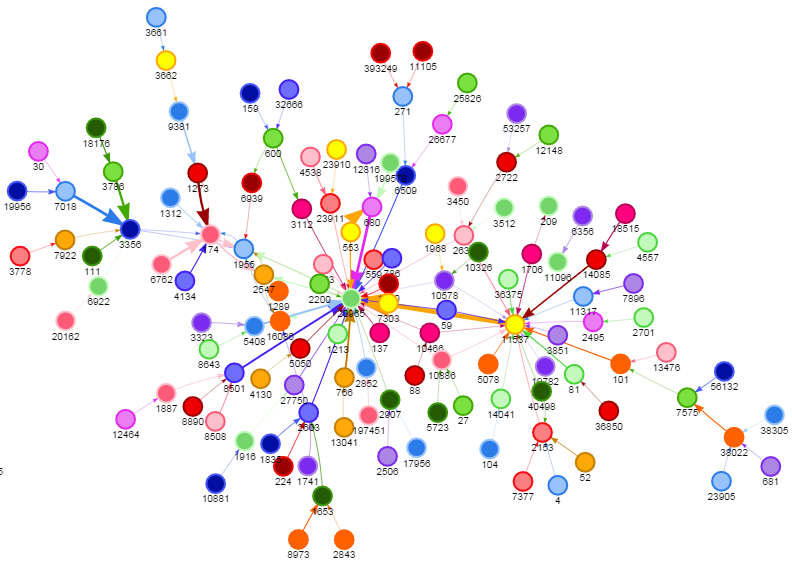
\includegraphics[width=1\textwidth,keepaspectratio]{figures/as-graph.png}

\end{document}
